\documentclass[journal]{IEEEtran}

\renewcommand{\baselinestretch}{1.0} % Change to 1.65 for double spacing
 
\usepackage{amsmath,amsfonts,amssymb}
\usepackage{graphicx}
\usepackage[colorlinks=true, allcolors=blue]{hyperref}


\usepackage{color}
\usepackage[latin9]{inputenc}
\usepackage{mathrsfs,amsmath}
\usepackage{graphicx}%
\usepackage{float}
\usepackage{amsfonts}%
\usepackage{amssymb}
\usepackage{braket}
\usepackage{bm}
%necessary for outline section of the article 
\usepackage{outline}

\newcommand{\mb}[1]{\bm{#1}}
\usepackage[T1]{fontenc}

\def\Nabla{\bm{\nabla}}
\def\bm{\mathbf}
\def\curl{\Nabla\times}
\def\div{\Nabla\cdot}
\def\lap{\Delta}
\def\vlap{\Delta}
\def\x{\hat{e}_{x}}
\def\y{\hat{e}_{y}}
\def\z{\hat{e}_{z}}
\def\p{\partial}
\def\h{\hat}
\def\tw{\tilde{\omega}}
\def\gm{\gamma}
\def\om{\omega}
\def\OM{\Omega}
\def\GM{\Gamma}
\def\dw{\delta\omega}
\def\dth{\Delta\theta}
\def\dk{\delta k}
\def\Hdth{\frac{\dth}{2}} %half Delta Theta
\DeclareMathOperator{\Tr}{Tr}


\title{Analysis of operating regimes of terahertz quantum cascade laser frequency combs}
\author{\IEEEauthorblockN{Petar Tzenov\IEEEauthorrefmark{1},
		David Burghoff\IEEEauthorrefmark{2},
		Qing Hu\IEEEauthorrefmark{2}, 
		Christian Jirauschek\IEEEauthorrefmark{1}}
	
	\IEEEauthorblockA{\IEEEauthorrefmark{1}Institute for Nanoelectronics, Technical University of Munich, D-80333 Munich, Germany}
	
	\IEEEauthorblockA{\IEEEauthorrefmark{2}Department of Electrical Engineering and Computer Science, Research Laboratory of Electronics, Massachusetts Institute of Technology, Cambridge, Massachusetts 02139, USA}
	\thanks{Corresponding author: P. Tzenov (email: petar.tzenov@tum.de ).}}



\IEEEtitleabstractindextext
 
\begin{document} 
\maketitle

	

\begin{abstract}
REWRITE REWRITE REWRITE -> overlaps with previous publication
Quantum cascade lasers (QCLs) promise to be efficient, cheap and compact sources of frequency combs in the mid- and far-infrared portions of the electromagnetic spectrum. Experimental results have shown comb generation in the mid-infrared as well as, more recently, the terahertz based on free running QCLs. The community appears to collectively agree that high order nonlinear optical processes, such as four wave mixing, are the main mode proliferation mechanisms that contribute to comb formation. In contrast, it has been argued that group velocity dispersion (GVD) is the thorn in the design of frequency combs as it leads to pulse broadening and limits the full exploitation of the gain bandwidth of the material. In the terahertz regime, the two widest comb generating devices demonstrated so far, have shown a strong variation of the beatnote?s linewidth with changing injection current, thus indicating that they experience "comb" regimes of operation that cover only a fraction of the whole dynamic range of these lasers. Here we present results from a coupled ensemble Monte-Carlo (EMC) and Maxwell-Bloch (MB) equations simulations of a terahertz quantum cascade laser frequency comb. We show that the correct compensation of group velocity dispersion is essential for the frequency stability of the laser in question and we also investigate the differences between comb and non-comb operation in the time domain. <-REWRITE REWRITE REWRITE 
\end{abstract}

\section{Introduction}

\section{Theoretical model}
The MB equations are a semi-classical model describing the light-matter interaction in microscopic systems, where the coherent coupling between the optical field and the gain medium is treated within a density matrix formalism, whereas the effect of the induced polarization onto the incident optical field is captured via the classical Maxwell's equations. This model is a generalization of the rate equations approach, which allows us to include optical nonlinearities and coherence effects into electron transport simulations and thus incorporate the physics of four wave mixing and resonant tunnelling into the system dynamics. We numerically solve the Maxwell-Bloch equations for a three level system with a single resonant tunnelling and a single optical transition included, whereas the physics of incoherent scattering mechanisms is treated phenomenologically via a rate equations approach. All the relevant scattering rates have been extracted by our ensemble Monte Carlo simulation code.

\subsection{Full perturbative solution}
In this section we will derive, based on perturbative expansion of the density matrix in powers of the incident electric field, analytical expressions of the first, second and third order susceptibilities in a three level quantum system. 

In its basic form the EOM can be written as 
\begin{align}
\frac{d\hat\rho}{dt} = -\frac{i}{\hbar}[\hat H,\hat\rho] + (\frac{d \rho }{dt}|_{coll}),
\end{align}
where $\rho$ is the density matrix, $H$ is the total Hamiltonian and the last term denotes phenomenologically included scattering rates. In our model, the Hamiltonian has two distinct contributions: $H_0$ for the bare system Hamiltonian, the eigenstates of which are the wave functions displayed in Fig. \ref{}, and the interaction Hamiltonian, $H_{int}$, modelling the effect of an applied electric field onto the system dynamics. Assuming a field $E_z$, polarized along the growth $z$-direction, it enters the Hamiltonian via the electric dipole approximation, i.e. $H_{int} = q_0 \hat{z} E_z$, where $\hat{z}$ denotes the position operator and $q_0$ the elementary charge. Due to the tunneling coupling between the injector and the upper laser level, the tight-binding eigenstates split into a doublet of "delocalized states", each coupled to the lower laser level via a dipole allowed transition. In fact, one can easily verify that the dipole matrix element between the upper and the lower level in the tight-binding basis, i.e. $d_{32}$, will be distributed amongst the dipole elements between each delocalized state and the lower level, i.e. $d_{\pm2}$, via the quadratic relation (see Appendix)
\begin{equation}
d_{32}^2 =d_{+2}^2+d_{-2}^2,
\end{equation} 
where the relative strength of the delocalized states' dipoles is determined by the detuning from "injector"-"upper level" resonance. In this dressed states/delocalized basis, we can write down the von Neumann equation as follows
\begin{align}
\label{eq:EOM_nm}
\dot{\rho}_{nm} = -i\omega_{nm}\rho_{nm}  - \frac{i}{\hbar} [H_{int},\rho]_{nm} + (\frac{d \rho }{dt}|_{coll})_{nm},
\end{align}
where $\omega_{nm} = (E_n-E_m)/\hbar$ is the transition frequency between levels $n$ and $m$ for $n,m \in\{+,-,2\}$. For the collision terms, we will assume the form 
\begin{align}
(\frac{d \rho }{dt}|_{coll})_{nm} = -\gamma_{nm}(\rho_{nm}-\rho_{nm}^{(eq)}),
\end{align}
with $\rho_{nm}^{(eq)}$ denoting the equilibrium value of the corresponding density matrix element and $\gamma_{nm}$ the convergence rate. Such an equilibrium state is governed by the pumping and depopulation mechanisms inherent from the QCL's active region design and, for the diagonal density matrix elements, $\rho_{nn}^{(eq)} = p_n$ describes the steady state electron distribution in the absence of electric field. For the off-diagonal elements, i.e. when $n\neq m$, we will assume that  $\rho_{nm}^{(eq)} = 0$. 

A standard technique for the analytical solution of Eq. (\ref{eq:EOM_nm}) is the perturbative expansion approach [cite], assuming a series expansion of the density matrix elements in powers of the electric field
\begin{equation}
\label{eq:expansion}
\rho_{nm} = \rho_{nm}^{(0)}+\rho_{nm}^{(1)}+\rho_{nm}^{(2)} +\rho_{nm}^{(3)} + ...
\end{equation} 
This approach is valid only for moderate strengths of the applied field and is a very good approximation for terahertz quantum cascade lasers due to the still relatively low output powers of these devices. We will solve Eq. (\ref{eq:EOM_nm}), assuming the solution form in Eq. (\ref{eq:expansion}), in a step-wise fashion, starting from the zero-th order element up to third order. This will allow us to derive explicit formulas for the linear, i.e. $\chi^{(1)}$, and higher order susceptibilities, i.e. $\chi^{(2)}$ and $\chi^{(3)}$, which govern the mode proliferation mechanisms in QCL frequency combs. Following Boyd [cite] we can now write the consecutive coupled differential equations as 
\begin{subequations}
\label{eq:EOM_expansion_nm}
\begin{align}
\dot{\rho}_{nm}^{(0)} &= -i\omega_{nm}\rho_{nm}^{(0)} -\gamma_{nm}(\rho_{nm}^{(0)}-\rho_{nm}^{(eq)}), \label{eq:EOM_zeroth}\\
\dot{\rho}_{nm}^{(1)} &= -(i\omega_{nm}+\gamma_{nm})\rho_{nm}^{(1)}  - i q_0E_z\hbar^{-1}[Z,\rho^{(0)}]_{nm}, \label{eq:EOM_first}\\
\dot{\rho}_{nm}^{(2)} &= -(i\omega_{nm}+\gamma_{nm})\rho_{nm}^{(2)}  - i q_0E_z\hbar^{-1}[Z,\rho^{(1)}]_{nm},  \label{eq:EOM_second}\\
\dot{\rho}_{nm}^{(3)} &= -(i\omega_{nm}+\gamma_{nm})\rho_{nm}^{(3)}  - i q_0E_z\hbar^{-1}[Z,\rho^{(2)}]_{nm},  \label{eq:EOM_third}
\end{align} 
\end{subequations}
where $Z$ denotes the position matrix in the delocalized basis and the other quantities are as defined previously.  
\subsection{First order susceptibility}
We start by explicit integration of Eqs. (\ref{eq:EOM_expansion_nm}). From the explicit form of the collision term in Eq. (\ref{eq:EOM_zeroth}) we can quickly deduce that $\rho_{nn}^{(0)} = \rho_{nn}^{(eq)} = p_n$ and $\rho_{nm}^{0} = 0$ for $n\neq m$. Putting that together we can write $\rho_{nm}^{(0)} = \delta_{nm}p_n $, where $\delta_{nm}$ is the Kronecker delta. Now, after we know these values we can plug the result in Eq. (\ref{eq:EOM_first}) and integrate. To do that we need to expand the electric field $E_z$ as a superposition of $M$ modes via
\begin{equation}
\label{eq:field_expansion}
E_z(t,x) = \frac{1}{2}(\sum_{j=1}^{M} A_j(t)u_j(x) e^{-i\omega_j t } + c.c.), \quad j \in N,
\end{equation}
where $j$ is the mode index and $\omega_j$  is the respective optical frequency, $A_j$ is the amplitude and $u_j$ is the longitudinal mode profile, assumed a complete set of orthogonal cavity eigenmodes. Assuming that the optical signal is relatively narrowband, distributed around some central frequency $\omega_c$ we can, with employing the rotating wave and slowly varying envelope approximations in hindsight, we rewrite Eq. (\ref{eq:field_expansion}) as 
\begin{align}
\label{eq:field_expansion_rwa}
E_z(t,x) &= \frac{1}{2}(e^{-i\omega_c t}\sum_{j=1}^{M} A_j(t)u_j(x) e^{-i(\omega_j-\omega_c) t } + c.c.) \nonumber \\
		&= \frac{1}{2}(e^{-i\omega_c t}\sum_{j=-q}^{p} A_j(t)u_j(x) e^{-i\tilde\omega_j t } + c.c.), 
\end{align}
where we have denoted with $\tilde \omega_j = \omega_j-\omega_c$ and have also changed the indexing, assuming $q$ modes with lower frequency than $\omega_c$ and $p$ modes with higher. Lastly, without loss of generality, we have also assumed that $\omega_c$, i.e. the central frequency, coincides with one of the cavity modes and has amplitude and longitudinal profile denoted by $A_0$ and $u_0$, respectively.   

Plugging in Eq. \ref{eq:field_expansion_rwa} into Eq. (\ref{eq:EOM_first}) and evaluating the commutator yields
\begin{align}
\label{eq:coherence_expansion}
\dot{\rho}_{nm}^{(1)} &= -i(\omega_{nm}+\gamma_{nm})\rho_{nm}^{(1)}  \nonumber \\ 
&- \frac{iq_0}{2\hbar}z_{nm}(p_m-p_n)(e^{-i\omega_c t}\sum_{j=-p}^{q}A_ju_je^{-\tilde\omega_j t} + c.c.).
\end{align}
Now setting $q_0z_{nm} = \mu_{nm}$ and also taking the ansatz $\rho_{nm}^{(1)} = \eta_{nm}^{(1)}e^{-i\omega_c t}$ for $nm = \pm2$, and employing the rotating wave approximation by retaining only slowly varying resonant terms
\begin{align}
\dot{\eta}_{nm}^{(1)} &= -i(\omega_{nm}-\omega_c+\gamma_{nm})\eta_{nm}^{(1)}  \nonumber \\ 
& + \frac{i\mu_{nm}}{2}(p_n-p_m)\sum_{j=-p}^{q}A_ju_je^{-\tilde\omega_j t}.
\end{align}
Explicit integration of the above expression, assuming time-constant field amplitudes $A_j$, yields
\begin{align}
\label{eq:nm_1_final}
\eta_{nm}^{(1)}(t)= \frac{\mu_{nm}}{2\hbar}(p_n-p_m) \sum_{j=-p}^{q}\frac{A_ju_je^{-\tilde\omega_j t}}{\omega_{nm}-\omega_c-\tilde{\omega_j}-i\gamma_{nm}}.
\end{align}

Note that within the rotating wave approximation, the only non-zero first order solutions are $\rho_{+2}^{(1)}$ and $\rho_{-2}^{(1)}$. Indeed, Eq. \ref{eq:coherence_expansion} tells us that $\rho_{nn}^{(1)} = 0 $ or at least will decay to zero with the rate $\gamma_{nn}$ whereas the rotating wave approximation has allowed us to neglect the coherence $\rho_{+-}^{(1)}$ due to the large values of the denominator upon explicit integration of Eq. \ref{eq:coherence_expansion}.  

To finally derive $\chi^{(1)}$ we compute the polarization via the expectation value of the dipole operator $\hat\mu = |q_0|\hat{z}$, i.e. 
\begin{align}
\label{eq:polarization_01}
P(t,x) &= -N_c<\hat \mu> = -N_c \Tr(\rho \mu)\nonumber \\
	&= -N_c\sum_{k=1}\Tr(\rho^{(k)}\mu),
\end{align}
where $N_c$ is the average carrier density and $\Tr$ is the trace. Expanding the polarization in powers of the electric field amplitude we can write 
\begin{align}
\label{eq:polarization_02}
P(t,x) &= P^{(1)}+P^{(2)}+P^{(3)} + ...,
\end{align}
where the first order term is given by 
\begin{align}
\label{eq:polarization_linear}
P^{(1)} &=  \frac{1}{2}e^{-i\omega_ct}\sum_{j}\epsilon_0 \chi^{(1)}(\tilde{\omega}_j) A_ju_je^{-i\tilde\omega_jt} + c.c..
\end{align}
Now taking Eqs. (\ref{eq:nm_1_final}) and (\ref{eq:polarization_linear}) and substituting for the first order term in Eq. (\ref{eq:polarization_01}) we obtain 
\begin{align}
\label{eq:polarization_linear_final}
\chi^{(1)}(\tilde\omega_j) &=  -\frac{N_c}{\epsilon_0\hbar}\sum_{n,m} \frac{\mu_{nm}^2(p_n-p_m)}{\omega_{nm}-\omega_c-\tilde{\omega_j}-i\gamma_{nm}}.
\end{align}


 


\subsection{Second order susceptibility}
In media with inversion symmetry the second order nonlinearity vanishes and thus $\chi^{(2)} = 0$. This condition is satisfied if the diagonal terms of the dipole matrix $Z$ are identically zero, which is a commonly assumed approximation in the theoretical treatment of QCLs. However, in reality this assumption is not satisfied since when biased quantum well heterostructures are highly assymetric along the growth direction and in fact are known to posses extremely large second order nonlinearities [cite]. Thus a necessary step towards more realistic modelling of these devices, especially in the context of comb generation, must be taken by including $\chi^{(2)}$ in the overall theoretical treatment. 

TODO: DERIVATION

\subsection{Third order susceptibility}
TODO: DERIVATION


\begin{figure*}[h!]
	\centering
	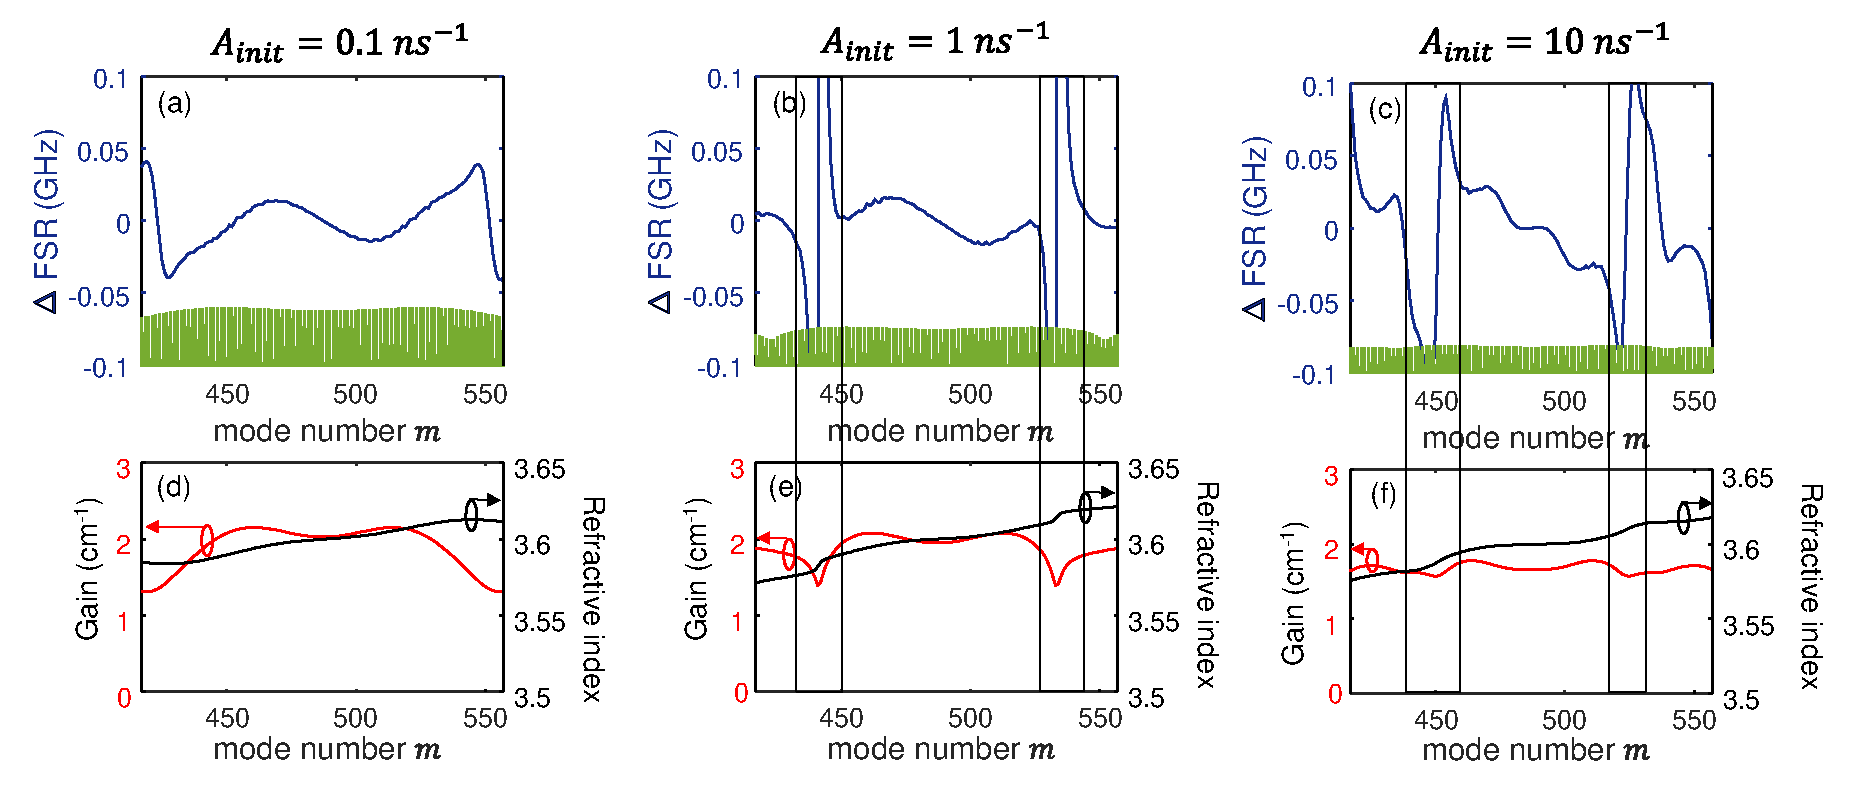
\includegraphics[width=0.95\textwidth]{IMGS/FSR_variation}
\end{figure*}

\section{Gain medium characterization}

A strong advantage of our model for the analysis of QCL frequency combs, in comparison to semi-analytical models introduced previously \cite{khurgin2014coherent,villares2015quantum}, is that it provides a relatively simplistic framework for the investigation and characterization of the QCL gain medium under different operating conditions. The lack of prior assumptions on the line spacing as well as the spatio-temporal evolution of the field modes, deprives us from the possibility of obtaining robust analytical results (due to the inherent complexity of the system of equations), however at the same time maintains the generality of the model. In our previous publication \cite{petz2016}, we have shown how we can emulate laboratory pump-probe experiments, such as THz time-domain spectroscopy, in order to extract valuable information about the complex refractive index, and from there all important derived quantities such as the spectral gain, the group velocity, the GVD coefficient and others. 

The general idea is to treat the gain medium of certain length $L$ as a nonlinear casual filter with some unknown transfer function $H(\omega)$. If were able to extract the magnitude and frequency response of this transfer function we could use this information to infer the real and complex part of the refractive indices. This can be done quite easily by simulating the passage of an unchirped pulse, e.g. a Gaussian with suitably chosen spectral width and amplitude, through the medium and recording the pulse at the output facet of the simulation region. The real power in this method lies in its universality as it allows us to characterize the time-dependent behaviour of the system under different operating conditions, by simply varying the model parameters.


In this section we use this computation trick in order to characterize the active region upon variation of the amplitude of the input pulse. In doing so, we can analyze the effects of different intensity-dependent phenomena, such as gain saturation and also self and cross-phase modulation, onto the system dynamics. More importantly, we show the non-trivial impact of the latter onto the cavity dispersion, which we believe provide an illustrative explanation on the reported failure of comb formation at high values of the injection current [cite].

For these simulations we analyze the dispersion of the QCL in Ref. \cite{burghoff2014terahertz}, with the aid of our model previously introduced in greater detail \cite{petz2016}. The assumed operating bias of the device is 11 kV/cm, a value at which we have calculated that the injector and the upper laser level (in the tight-binding approximation) are perfectly aligned. As we have already showed, this ought to result in a symmetric gain with negligible second order dispersion. 


 



 




\section{Mode proliferation mechanisms}
It has been experimentally [cite] and also theoretically [cite] demonstrated that four wave mixing (FWM) acts as the main comb proliferation mechanism in mid-IR and THz QCLs due to their strong third order nonlinearity.  Experimental pump-probe techniques have been used to classify the nature of the FWM process and it has been shown that namely degenerate FWM, where two pump signals combine nonlinearly to produce a scattered Stokes and anti-Stokes frequencies, is at play in such devices (Fig. 2a, b). To verify if our computational model captures those effects, we have emulated those experiments and the corresponding results can be seen in Fig. 2c, d.  Furthermore, we used the same method to generate a 2D contour plot of the third order susceptibility, which can be seen in Fig. 2e.  

\section{Comb degradation mechanisms}
It has been argued that group velocity dispersion (GVD) has an extremely detrimental effect onto the comb coherence. In fact, for THz QCLs one has to go employ sophisticated dispersion compensation mechanisms (DCM) in order to undo the signal distortion caused by GVD [cite].  Only successfully compensated QCLs would emit a stable frequency comb (Fig. 3a), characterized by a broad optical spectrum and a strong narrow beatnote signal (Fig. 3b). In order to investigate the importance of a correct DCM, we simulated the device in [cite]. Numerically, the dispersion compensation was performed in the frequency domain by subtracting a previously recorded higher order phase (see upper left inset of Fig. 1) from the total phase acquired by the signal. We see that the correctly compensated dispersion reduces the signal to noise ratio in the beatnote while still maintaining multimode emission, both in experiment, Fig.3b, and simulation, Fig. 4b. In contrast, simulations without DCM yielded a highly noisy and chaotic beatnote signal, with two distinct peaks, probably corresponding to the round trip frequency of the high and low lobe signals. 

In the time domain, due to the strongly anticrossed gain, a transient pulse switching behaviour between high and low frequency lobe?s instantaneous intensities has been observed, Fig. 3a [cite]. Our simulations could reproduce this ?temporal hole burning? effect. It is worthwhile to note that, due to the equilibrated group velocity of the high and low freq. lobe pulses, their shape was preserved over many hundreds of round trips, Fig. 4a. In comparison, when dispersion was not compensated for, the pulse switching behaviour persisted, however with more chaotic time profile, Fig. 4c, evolving from round trip to round trip, which is probably a time domain manifestation of the chaotic beatnote signal.  

\section{Long-time simulations of quantum cascade laser based THz combs}

\section{Conclusion}
We have presented a theoretical model suitable for the simulation of THz QCLs in comb and non-comb regimes of operation, based on the full numerical solution of the Maxwell-Bloch equations in rotating wave approximation. We have shown that our approach correctly captures the complicated dynamics between four wave mixing, coherent tunneling and spectral gain splitting, group velocity dispersion, as well as spatial hole burning, as it delivers simulation results in good agreement with experimental data. We have used this model to characterize the spectral gain profile and the corresponding group velocity delay, and to investigate the FWM as the dominant comb proliferation mechanism. Simulations of comb operation yielded a spectral comb shape in good agreement with experiment, and the temporal switching behaviour between the high and low frequency components reported in experiment could also be reproduced. Furthermore, we have demonstrated that in contrast to earlier theoretical approaches our model can also capture non-ideal comb operation and transitions between comb and non-comb operating regimes.



% References <- adhere to respective journal style 
\bibliographystyle{IEEEtran}
\bibliography{D:/docs/MAIN-PROJECTS/PAPERS/literature/bib_resources}


\end{document} 
